% Quantifying Target-Domain Data Requirements for Object Detection under Domain Shift
% IEEE conference format (IEEEtran). Compile with pdfLaTeX + BibTeX (Overleaf default).
\documentclass[conference]{IEEEtran}
\IEEEoverridecommandlockouts

\usepackage{cite}
\usepackage{amsmath,amssymb}
\usepackage{graphicx}
\usepackage{booktabs}
\usepackage{multirow}
\usepackage{array}
\usepackage{xspace}
\usepackage{textcomp}
\usepackage{url}
\usepackage[hidelinks]{hyperref}

\graphicspath{{figures/}}

% ---------------------------------------------------------------------------
% Notation used throughout the paper
% ---------------------------------------------------------------------------
\newcommand{\NBE}{\ensuremath{N_{\mathrm{BE}}}\xspace}        % break-even budget
\newcommand{\Nsf}{\ensuremath{N_{75}}\xspace}                 % 75% recovery threshold
\newcommand{\Nnf}{\ensuremath{N_{90}}\xspace}                 % 90% recovery threshold
\newcommand{\Nx}{\ensuremath{N_{\times}}\xspace}              % crossover budget
\newcommand{\Neq}{\ensuremath{N_{\mathrm{eq}}}\xspace}        % equivalent labeled budget
\newcommand{\mAPc}{\ensuremath{\mathrm{mAP}_{c}}\xspace}      % target ceiling
\newcommand{\mAPsrc}{\ensuremath{\mathrm{mAP}_{\mathrm{source}}}\xspace}
\newcommand{\mAPzero}{\ensuremath{\mathrm{mAP}(0)}\xspace}    % zero-shot
\newcommand{\aldi}{ALDI\texttt{++}\xspace}

% Note set under a table, full width of the float, justified.
\newcommand{\tabnote}[1]{\par\vspace{2pt}\parbox{\linewidth}{\footnotesize #1}}
% Framed statement of the main claim.
\newcommand{\claimbox}[1]{\par\medskip\noindent\fbox{\parbox{\dimexpr\linewidth-2\fboxsep-2\fboxrule\relax}{#1}}\par\medskip}

\begin{document}

\title{Quantifying Target-Domain Data Requirements for Object Detection under Domain Shift:\\
Most of the Small-Budget Advantage of Domain Adaptation over Fine-Tuning Is Not Adaptation}

% TODO: fill in the author block before submission.
\author{\IEEEauthorblockN{Author Names}
\IEEEauthorblockA{Affiliation\\
City, Country\\
email@example.com}}

\maketitle

\begin{abstract}
How many labeled target-domain images does an object detector need to recover from domain shift, and when does a domain adaptive method pay off over plain fine-tuning on those images? We train a Faster R-CNN R50-FPN detector on daytime, clear-weather BDD100K images and study three target domains: night and clear (lighting), day and rainy (weather), and night and rainy (compound). The main result comes from a control arm. We compare \aldi, a domain adaptive object detection (DAOD) method, with fine-tuning (FT) on the same nested labeled subsets, and add a replay control that keeps everything from \aldi (source-image mixing, strong augmentation, EMA teacher) but drops the unlabeled target stream and the distillation, that is, the adaptation. At the two budgets tested, $N = 10$ and $N = 100$ labeled images, the replay control reproduces 76--94\% of \aldi's advantage over FT in all three shifts, with three seeds and every lower 95\% confidence bound above 0.5: at small labeled budgets, most of the advantage of domain adaptation over fine-tuning is not adaptation. At $N = 10$ that advantage is mostly the avoidance of the damage FT does by overfitting; against the source model, \aldi gains only 0.003--0.011 AP. At $N = 1{,}000$, with labeled image passes matched, FT leads \aldi on lighting (by 0.008 AP) and compound (by 0.007 AP), and there is no meaningful difference on weather; distillation contributes nothing at this budget. The data-efficiency curves are the context that makes this measurable: under a fixed schedule, FT is worse than zero-shot for $N \leq 50$, breaks even at $N = 100$--$250$, and reaches 75\% recovery at $N = 5{,}000$ (lighting) and $N = 1{,}000$ (compound). A 12-epoch ceiling is not materially higher than the 3-epoch one in any shift. For lighting and compound the thresholds barely move: the lighting \Nnf moves from 10,000 to the full pool of 18,015, and the compound \Nnf from not determined within the pool to 1,738. Weather leaves only 0.015 AP to recover against the 3-epoch ceiling (0.011 AP against the 12-epoch ceiling, under which all its thresholds are undetermined), so it serves as a third replication of the decomposition, not as a third threshold measurement.
\end{abstract}

\begin{IEEEkeywords}
object detection, domain shift, domain adaptation, label efficiency, fine-tuning, BDD100K
\end{IEEEkeywords}

% Sections 1 (Introduction) and 2 (Related work).

\section{Introduction}\label{sec:intro}

A detector trained under one condition often loses performance when it is deployed under another: night instead of day, rain instead of clear weather. Labeling images of a new domain is expensive, so the practical question has two parts: how many labeled target-domain images are needed to recover, and when a domain adaptive object detection (DAOD) method is worth more than simple fine-tuning on those same images.

DAOD papers usually report an advantage over a baseline. ALDI (Kay et al.~\cite{kay2024aldi}) showed that the reported advantage depends strongly on implementation choices and on how the baseline is built. This study continues in that direction, in the setting where target labels are available: besides comparing \aldi with fine-tuning (FT), we run a control arm that keeps the training recipe of \aldi unchanged but removes the adaptation. The difference between \aldi and the control arm is the part due to adaptation; the difference between the control arm and FT is the part due to the training recipe.

The contributions of this paper, in order of importance, are:
\begin{enumerate}
\item \textbf{Decomposition with a control arm.} At $N = 10$ and $N = 100$, most of the advantage of \aldi over FT is reproduced by an arm without adaptation, in all three shifts. At $N = 1{,}000$, after the number of labeled image passes is matched, FT leads on lighting and compound. Others can verify this claim, because it only requires adding one control arm to any DAOD comparison.
\item \textbf{Data-efficiency curves} for the three shifts on the same fixed test sets, with recovery normalized by the target-domain ceiling. They are the context: it is the shape of the FT curve at small $N$ that produces most of the advantage of \aldi.
\item \textbf{Practical thresholds} \NBE (break-even), \Nsf and \Nnf, reported against both the 3-epoch ceiling and the 12-epoch ceiling, with ladder intervals and confidence intervals (CIs). These are secondary results.
\item \textbf{Side results:} the amount of source forgetting after fine-tuning, and a control with COCO initialization instead of initialization from the source model.
\end{enumerate}
Section and table titles refer to five research questions: how much each shift reduces accuracy (RQ1, Section~\ref{sec:drop}), how recovery grows with the labeled budget (RQ2, Section~\ref{sec:recovery}), the labeled-budget thresholds (RQ3, Section~\ref{sec:thr-two}), whether the shifts differ at the same pool size (RQ4, Section~\ref{sec:rq4}), and how a DAOD method compares with fine-tuning (RQ5, Section~\ref{sec:main}).

This paper does not aim to show that domain shift degrades detector performance, nor does it propose another day$\to$night benchmark on BDD100K; both have already been studied.

This paper extends an earlier version (8 November 2026) with 42 runs added after a review on 21 November 2026: the 12-epoch ceiling, the matched-passes experiment at $N = 1{,}000$, and additional seeds for the control arm. The main rules for reading the results of these runs were written down before the runs were scored; Section~\ref{sec:rules} lists the rules that were set afterwards.

\section{Related Work}\label{sec:related}

\textbf{Domain adaptation for object detection.} Most DAOD methods with public code are built on Faster R-CNN (Ren et al.~\cite{ren2015faster}). Methods of the mean-teacher family (Tarvainen and Valpola~\cite{tarvainen2017mean}), such as Adaptive Teacher (Li et al.~\cite{li2022adaptive}) and MIC (Hoyer et al.~\cite{hoyer2023mic}), use a teacher updated by an exponential moving average (EMA) to produce pseudo-labels or distillation targets on unlabeled target images. ALDI (Kay et al.~\cite{kay2024aldi}) reimplements many methods in a common framework on Faster R-CNN R50-FPN, compares them with a fairly trained source baseline, and proposes \aldi. We chose \aldi because it uses exactly the same architecture as this study and is the strongest configuration in that benchmark.

\textbf{Adaptation with little labeled target data.} Few-shot Adaptive Faster R-CNN (Wang et al.~\cite{wang2019fewshot}) and AcroFOD (Gao et al.~\cite{gao2022acrofod}) adapt a detector with a small number of labeled target images; AcroFOD evaluates several amounts of target data in some settings and compares against a fine-tuning baseline. Few-shot detection benchmarks measure absolute performance at fixed numbers of shots per class, on novel classes, so they do not answer the question asked here: what fraction of the performance attainable in the target domain a labeled budget recovers.

\textbf{BDD100K} (Yu et al.~\cite{yu2020bdd100k}) has been used as a target domain in studies of domain adaptation for detectors (e.g., Hsu et al.~\cite{hsu2020progressive}), including day$\to$night adaptation and adaptation across weather conditions. The gap this study targets is narrower: hold one real dataset and one test set fixed, vary the target labeled budget over a wide range, and split the advantage of a DAOD method into a part due to adaptation and a part due to the training recipe.

% ===========================================================================
% Section 3: Data and evaluation protocol; Section 4: Method
% ===========================================================================

\section{Data and Evaluation Protocol}\label{sec:data}

\subsection{Split and Domains}\label{sec:split}

The original BDD100K train folder has 69,863 images with detection labels. They were split once, with seed 20260916, into 55,000 train images and 14,863 held-out test images, stratified jointly by time of day, weather and scene type. The official validation set (val, 10,000 images) is kept unchanged. The public 20,000-image test set has no detection labels and is therefore not used. The membership of each split is frozen by manifests and SHA256 hashes. No image is shared between splits, either by file name or by content.

The source domain is daytime with clear weather. The three target domains form a $2\times2$ design over time of day and weather (Table~\ref{tab:domains}): lighting changes only the illumination, weather changes only the weather, and compound changes both.

\begin{table}[t]
\centering
\caption{Domains and split sizes.}
\label{tab:domains}
\footnotesize
\setlength{\tabcolsep}{3pt}
\begin{tabular}{@{}l>{\raggedright\arraybackslash}p{0.52in}r>{\raggedright\arraybackslash}p{0.75in}>{\raggedright\arraybackslash}p{1.0in}@{}}
\toprule
Domain & Condition & \begin{tabular}[t]{@{}r@{}}Train\\pool\end{tabular} & Final test & Selection val \\
\midrule
source   & daytime, clear & 9,804  & 2,650 & 1,764 (source checkpoint selection) \\
lighting & night, clear   & 18,015 & 4,869 & 3,274 (schedule pilot only) \\
weather  & daytime, rainy & 1,985  & 933 (537 test + 396 val) & none \\
compound & night, rainy   & 1,738  & 756 (470 test + 286 val) & none \\
\bottomrule
\end{tabular}
\end{table}

The val images of weather and compound were moved into the final test set, because the original test sets of these two domains (537 and 470 images) were below the minimum of 600 images. As a consequence, weather and compound have \textbf{no val set for selection}; every target-domain run keeps the final update of a fixed schedule instead of selecting a checkpoint.

\subsection{Labels}\label{sec:labels}

The labels are the 2018 BDD100K detection release, obtained through the \texttt{solesensei\_bdd100k} mirror on Kaggle; every image and label file matches the mirror in size and CRC32. The 2018 release has been superseded by the Detection 2020 labels (\texttt{det\_20}). Keeping the 2018 release is a recorded decision, and it is stated among the limitations (Section~\ref{sec:limitations}). The legacy class names (person, bike, motor) are mapped to the canonical names.

\subsection{Zero-Shot Gate}\label{sec:gate}

Before any ladder was run, the zero-shot gap of each shift was measured with the source model: source val versus the target domain's train pool, which the model had never seen, so no test label was read. A shift whose 95\% CI does not exceed 0.01 AP is flagged. All three shifts pass the gate (Table~\ref{tab:gate}).

\begin{table}[t]
\centering
\caption{Zero-shot gate (source val versus the target train pool, 1,000 bootstrap resamples).}
\label{tab:gate}
\footnotesize
\setlength{\tabcolsep}{3pt}
\begin{tabular}{@{}lcc@{}}
\toprule
Shift & Zero-shot gap (AP) & 95\% CI \\
\midrule
lighting & 0.100 & 0.091--0.110 \\
weather  & 0.032 & 0.024--0.041 \\
compound & 0.129 & 0.121--0.139 \\
\bottomrule
\end{tabular}
\end{table}

Weather passes the gate, but with the smallest gap. Every weather result is therefore reported with its CI and the raw change in AP.

\subsection{Test-Label Access}\label{sec:testaccess}

No run reads test labels during training; the manifest of each run records this. After a group of runs has finished, all of the group's prediction files are frozen in a plan (with the hash of every file and every checkpoint), and that plan is then scored exactly once. There are three plans (Table~\ref{tab:plans}).

\begin{table}[t]
\centering
\caption{The three frozen plans, each scored exactly once.}
\label{tab:plans}
\footnotesize
\setlength{\tabcolsep}{3pt}
\begin{tabular}{@{}l>{\raggedright\arraybackslash}p{1.25in}cl@{}}
\toprule
Plan & Contents & \begin{tabular}[t]{@{}c@{}}Prediction\\sets\end{tabular} & Scored on \\
\midrule
campaign      & fine-tuning, 3-epoch ceiling, COCO control & 87 & 6 Nov.~2026 \\
RQ5           & \aldi and replay under the original rules & 46 & 7 Nov.~2026 \\
supplementary & 12-epoch ceiling, additional replay seeds, matched-passes experiment & 42 & 23 Nov.~2026 \\
\bottomrule
\end{tabular}
\end{table}

All three plans use the same 1,000 test-image resamples (seed 20261030), so every comparison between arms is paired on the same resamples.

\section{Method}\label{sec:method}

\subsection{Detector and Source Model}\label{sec:detector}

The detector is Faster R-CNN with a ResNet-50 FPN backbone (Lin et al.~\cite{lin2017fpn}; the torchvision implementation), initialized from COCO (Lin et al.~\cite{lin2014coco}) and run at the native resolution of $1280\times720$ (\texttt{min\_size=720}, \texttt{max\_size=1280}). This architecture was chosen because of RQ5: almost every public DAOD implementation targets Faster R-CNN, so choosing it keeps a comparison with an adaptation method feasible.

The source model is trained once on the 9,804 source images: 12 epochs, batch 4, automatic mixed precision (AMP), learning rate (LR) 0.005, a warmup of 500 updates, 29,412 updates in total (about 118,000 image passes). The checkpoint is selected on source val only; the selected checkpoint is the final update, with a reliable mAP$_{50:95}$ of 0.352 on source val and 0.342 on source test. Every target-domain arm is initialized from this same checkpoint.

\subsection{Fine-Tuning Schedule}\label{sec:schedule}

Every target-domain fine-tuning run (the budget rungs, the ceilings, the controls) uses one shared rule: train for $\max(S \text{ updates}, E \text{ epochs})$ on the $N$ sampled images, then keep the final update. The fixed settings are batch 2, SGD with momentum 0.9, weight decay $5\cdot10^{-4}$, LR $10^{-3}$, a warmup of 50 updates followed by cosine decay to 1\% of the LR, gradient clipping at 10, and AMP.

The values of $S$ and $E$ were fixed by a pilot on lighting val only, under a rule written before the pilot ran: take the largest $S$ and the smallest $E$ that lie within $\delta = 0.005$ AP of the best configuration. The result is \textbf{\boldmath $S = 500$, $E = 3$}. The value $E = 3$ was chosen by a very thin margin: $E = 2$ trails $E = 5$ by exactly 0.00511 AP, that is, it lies outside $\delta$ by only 0.0001. Consequences of the rule:
\begin{itemize}
\item $N \leq 333$ receives 500 updates; for $N = 10$ this is equivalent to about 100 epochs.
\item $N \geq 500$ receives $1.5\cdot N$ updates (3 epochs at batch 2).
\item The pilot already indicated that at $N = 10$, fine-tuning makes the model 0.05--0.06 AP worse than the source model. This is recorded as a result, not as a reason to retune the schedule.
\end{itemize}

\subsection{Budget Ladder, Ceilings and Controls}\label{sec:ladder}

\begin{itemize}
\item \textbf{Ladder:} $N = 10$, 25, 50, 100, 250, 500, 1,000 and the full pool; lighting additionally has 2,000, 5,000 and 10,000. Every rung below the full pool has 3 sampling seeds (0, 1, 2), nested by seed: for the same seed, the $N = 25$ sample contains the $N = 10$ sample.
\item \textbf{3-epoch ceiling:} fine-tuning on the full pool under exactly the schedule above, 2 seeds. This is the top rung of the ladder.
\item \textbf{12-epoch ceiling} (added in response to the review): full pool, 12 epochs (the same number of epochs as the source model), 2 seeds, every other setting unchanged. On lighting it is 108,096 updates, about 216,000 image passes, compared with about 54,000 for the 3-epoch ceiling.
\item \textbf{Matched pool of 1,738 images} (for RQ4): the lighting and weather ceilings are recomputed at the pool size of compound, for both the 3-epoch and the 12-epoch ceiling, 2 seeds.
\item \textbf{COCO-initialization control:} at $N = 100$ and $N = 1{,}000$, the same run but initialized from the COCO weights instead of the source model, seed 0.
\end{itemize}

\subsection{Metric, Recovery and Thresholds}\label{sec:metrics}

\textbf{The primary metric} is mAP$_{50:95}$ averaged over a class roster that is fixed for every domain: pedestrian, car, traffic light, traffic sign (called \emph{reliable mAP}). These are the four classes with the most instances in all four domains; the metric is undefined if a class is missing. The 10-class mean is a sensitivity analysis. Every score goes through a single evaluation path (pycocotools).

\textbf{Drop} is defined as
\begin{equation}
\mathrm{Drop} = \mAPsrc - \mAPzero,
\label{eq:drop}
\end{equation}
where \mAPsrc is the score of the source model on source test and \mAPzero is the score of the source model on the target domain's test set (zero-shot).

\textbf{Recovery(\boldmath$N$)} is defined as
\begin{equation}
\mathrm{Recovery}(N) = \frac{\mathrm{mAP}(N) - \mAPzero}{\mAPc - \mAPzero},
\label{eq:recovery}
\end{equation}
where \mAPc is the target-domain ceiling, not \mAPsrc. A target domain can be intrinsically harder than the source domain (night is harder than day), so normalizing by \mAPsrc would mix the domain gap with intrinsic difficulty. Recovery is not clipped: a negative value means that fine-tuning is worse than zero-shot. The minimum denominator is 0.01 AP; when more than 5\% of the bootstrap resamples have a denominator below this level, recovery and the thresholds are recorded as \emph{undetermined}, together with the number of such resamples.

\textbf{Thresholds} are defined in a sustained sense on the recovery curve averaged over seeds:
\begin{itemize}
\item \NBE: the smallest rung $N > 0$ at and above which recovery is always $> 0$ (break-even).
\item \Nsf, \Nnf: the smallest rung $N$ at and above which recovery is always $\geq 0.75$ or $\geq 0.90$, respectively.
\item A threshold that is reached only at the ceiling rung itself (where recovery equals 1 by definition) is recorded as \textbf{not determined within the pool}, together with the largest rung that has not reached it. The $N_{95}$ threshold of our original study proposal has been dropped, because it falls into exactly this case in all three shifts.
\end{itemize}

\textbf{Uncertainty} is estimated with a hierarchical bootstrap: test images are resampled (1,000 times, seed 20261030) and sampling seeds are resampled; the seed-to-seed variation of the ceiling is also propagated into the denominator. The interval of each threshold is taken from the 95\% CI band of the recovery curve.

\textbf{The RQ1 interaction} is $\mathrm{Drop}(\text{compound}) - \mathrm{Drop}(\text{lighting}) - \mathrm{Drop}(\text{weather})$. Besides the CI, we report the minimum detectable interaction, $(z_{0.975} + z_{0.80})\cdot\mathrm{SE}$ (SE is the bootstrap standard deviation), both in AP and as a fraction of the weather effect.

\textbf{The log-linear fit},
\begin{equation}
\mathrm{Recovery} = \alpha + \beta\cdot\ln N,
\label{eq:fit}
\end{equation}
is used only for interpolation. The fit region runs from the first rung whose lower CI bound is above 0 (and stays so at every larger rung) to the largest rung below the ceiling; at least 4 rungs are required. $R^2$ and RMSE are computed on the fit region only. A threshold from the fit is reported only when it lies within the corresponding ladder interval. Held-out check: the fit is made on the three lowest rungs of the region and predicts the remaining rungs.

\subsection{\texorpdfstring{\aldi}{ALDI++} and the Replay Control Arm}\label{sec:aldi}

\aldi was reimplemented in torchvision from the paper and the published configuration files (the original code repository has no license, so its code was not copied). The configuration follows \aldi: an EMA teacher; labeled images receive strong augmentation and random erasing; on unlabeled images, the student receives strong augmentation plus MIC-style block masking (ratio 0.5, 32 px blocks), and the teacher receives a weakly augmented version; soft distillation on all four outputs (classification and regression of the ROI head, objectness and regression of the RPN); hard pseudo-labels (threshold 0.8) used only for anchor and proposal sampling; no feature alignment; the scored model is the EMA teacher.

\textbf{Differences from the original \aldi:} fixed $1280\times720$ images (no multi-scale training); no separate burn-in stage, because every arm is initialized from the same source model as FT; a small batch, 2 labeled and 2 unlabeled images per step, with LR $10^{-3}$ as for FT; the use of labeled target images (semi-supervised) is our extension, since the original ALDI uses no target labels.

\begin{table}[t]
\centering
\caption{The arms of RQ5. The adapt arm is \aldi; the replay arm keeps everything from the adapt arm except the adaptation.}
\label{tab:arms}
\footnotesize
\setlength{\tabcolsep}{3pt}
\begin{tabular}{@{}>{\raggedright\arraybackslash}p{0.6in}>{\raggedright\arraybackslash}p{0.95in}>{\raggedright\arraybackslash}p{0.85in}>{\raggedright\arraybackslash}p{0.75in}@{}}
\toprule
Arm & Labeled stream (2 images/step) & Unlabeled stream (2 images/step) & Updates \\
\midrule
FT & 2 labeled target images & none & max(500, 3~epochs) \\
adapt, $N = 0$ & 2 source images & full target pool, labels hidden & 2,000 \\
adapt, $N > 0$ & 1 source image + 1 of the $N$ labeled target images & full target pool & max(2,000, $2N$) \\
replay (control) & as adapt & none, no distillation & as adapt \\
\bottomrule
\end{tabular}
\end{table}

The replay arm (Table~\ref{tab:arms}) still mixes in source images and still uses strong augmentation and the EMA teacher; it drops only the unlabeled target stream and the distillation. Therefore:
\begin{itemize}
\item \textbf{adapt $-$ replay} is the value of distillation on unlabeled target images, that is, the adaptation part;
\item \textbf{replay $-$ FT} is the value of the training recipe (source-image mixing, strong augmentation, EMA).
\end{itemize}

Two parameters of \aldi were fixed by a pilot on lighting val only, under a rule written in advance: the EMA decay $\alpha = 0.9996$ and $T = 2{,}000$ updates. The run length is $\max(T, 2N)$. The original grid has 46 runs: adapt at $N = 0$ (2 seeds per shift), semi-supervised adapt at $N = 10$, 100 and 1,000 (plus 5,000 for lighting) with 3 seeds and exactly the nested subsets of FT, and replay with seed 0 at $N = 0$, 10, 100 and 1,000.

\textbf{Supplementary runs added in response to the review (30 runs):} replay with the additional seeds 1 and 2 at $N = 10$ and 100 (12 runs); adapt and replay at $N = 1{,}000$ with 3,000 updates instead of 2,000, 3 seeds (18 runs). With 3,000 updates and 1 labeled target image per step, the number of labeled target image passes equals that of FT at $N = 1{,}000$ (1,500 updates $\times$ 2 images $=$ 3,000 passes). This is the \emph{matched-passes experiment}.

\subsection{RQ5 Quantities}\label{sec:rq5quant}

\begin{itemize}
\item \textbf{\boldmath$\Delta(N)$} $=$ \aldi $-$ FT, paired by sampling seed; an advantage is meaningful when $\Delta \geq 0.005$ and the lower bound of the 95\% CI is $> 0$.
\item \textbf{Crossover \boldmath\Nx:} the smallest rung $N$ from which \aldi no longer has a meaningful advantage at any larger rung.
\item \textbf{Equivalent budget \boldmath\Neq:} the number of images FT needs to reach the same mAP as \aldi, interpolated linearly in $\log N$ at the sustained crossing of the FT curve.
\item \textbf{Replay share} $= (\text{replay} - \text{FT}) / (\text{adapt} - \text{FT})$: the part of the advantage of \aldi over FT that an arm without adaptation reproduces. It is paired by seed over the seeds common to the three arms; it is undetermined when $|\text{adapt} - \text{FT}| < 0.005$, and it is not quoted when more than 5\% of the bootstrap resamples fall into that case.
\item \textbf{Against the source model:} because FT at $N \leq 50$ is below even zero-shot, the same decomposition is recomputed with the source model as the reference, $(\text{replay} - \mAPzero) / (\text{adapt} - \mAPzero)$.
\end{itemize}

\subsection{Which Rules Were Written in Advance and Which Were Set Later}\label{sec:rules}

This distinction determines how much confidence each conclusion deserves, so it is stated separately (Table~\ref{tab:rules}).

\begin{table}[t]
\centering
\caption{Status of the analysis rules.}
\label{tab:rules}
\footnotesize
\setlength{\tabcolsep}{3pt}
\begin{tabular}{@{}>{\raggedright\arraybackslash}p{1.4in}>{\raggedright\arraybackslash}p{0.95in}>{\raggedright\arraybackslash}p{0.75in}@{}}
\toprule
Rule & When written & Nature \\
\midrule
FT schedule ($S$, $E$, LR); $\alpha$ and $T$ of \aldi & before the pilot & pre-registered \\
Definitions of $\Delta$, \Nx, \Neq; seed-0 decomposition & before the RQ5 grid & pre-registered \\
12-epoch ceiling as the denominator regardless of the result; the ``materially higher'' criterion; the reading rule for the matched-passes experiment; the rule for the main claim & 21 Nov., before the supplementary runs were scored, after the original grid had been seen & descriptive; the independent confirmation is new data \\
Log-linear fit region; interaction detection limit; replay share & 21 Nov., after the curves had been seen & descriptive \\
Recovery undetermined when $>5\%$ of bootstrap resamples are undetermined; the two ceilings presented side by side & 23 Nov., after the supplementary results had been seen & descriptive \\
Sustained crossing when computing \Neq & during the analysis of the RQ5 grid & descriptive \\
\bottomrule
\end{tabular}
\end{table}

The rule for the main claim, specifically, was written after the replay share at seed 0 had been seen (0.82--0.95 at $N = 10$ and 0.78--0.86 at $N = 100$). Its independent confirmation therefore comes from the two new seeds of the replay arm.

% ===========================================================================
% Section 5: Main result -- which part of the DAOD advantage is adaptation
% ===========================================================================
\section{Main Result: Which Part of the DAOD Advantage Is Adaptation}\label{sec:main}

\subsection{\texorpdfstring{\aldi}{ALDI++} versus Fine-Tuning}\label{sec:aldi-vs-ft}

\begin{table*}[t]
\centering
\caption{$\Delta(N) = {}$\aldi $-$ FT, reliable mAP$_{50:95}$, mean over seeds (95\% CI). At $N = 0$, the baseline is zero-shot.}
\label{tab:delta}
\footnotesize
\setlength{\tabcolsep}{3pt}
\begin{tabular}{@{}lccccc@{}}
\toprule
Shift & $N = 0$ & $N = 10$ & $N = 100$ & $N = 1{,}000$ & $N = 5{,}000$ \\
\midrule
lighting & \textbf{+0.009} (0.008, 0.011) & \textbf{+0.070} (0.068, 0.073) & \textbf{+0.015} (0.014, 0.017) & $-$0.011 ($-$0.012, $-$0.009) & $-$0.010 ($-$0.011, $-$0.008) \\
weather & \textbf{+0.006} (0.003, 0.007) & \textbf{+0.057} (0.050, 0.066) & \textbf{+0.014} (0.009, 0.019) & $-$0.003 ($-$0.005, $-$0.001) & \\
compound & \textbf{+0.011} (0.008, 0.014) & \textbf{+0.061} (0.054, 0.068) & \textbf{+0.016} (0.012, 0.019) & $-$0.012 ($-$0.014, $-$0.009) & \\
\bottomrule
\end{tabular}
\tabnote{Bold: an advantage that is meaningful under the rule. Weather at $N = 0$ only just passes the threshold (0.0055). At $N = 1{,}000$ the \aldi runs are the original 2,000-update runs; the results after matching are in Section~\ref{sec:matched}.}
\end{table*}

Table~\ref{tab:delta} gives $\Delta(N)$ for each shift and budget. Under the original rule, the crossover \Nx lies in the interval $(100, 1{,}000]$ in all three shifts. The \aldi curve is almost flat: from $N = 0$ to $N = 1{,}000$ it rises by only 0.003--0.010 AP, whereas the FT curve is much steeper after the overfitting region at small $N$ (Table~\ref{tab:abs}, Figs.~\ref{fig:rq5-lighting}--\ref{fig:rq5-weather}).

\begin{table}[t]
\centering
\caption{Absolute mAP (reliable, mean over seeds). DA is \aldi with the original number of updates.}
\label{tab:abs}
\footnotesize
\setlength{\tabcolsep}{3pt}
\begin{tabular}{@{}lcccccccc@{}}
\toprule
 & & \multicolumn{4}{c}{DA at $N$} & \multicolumn{2}{c}{FT at $N$} & FT \\
\cmidrule(lr){3-6}\cmidrule(lr){7-8}\cmidrule(l){9-9}
Shift & zero-shot & 0 & 10 & 100 & 1,000 & 100 & 1,000 & \begin{tabular}[b]{@{}c@{}}full pool,\\3 epochs\end{tabular} \\
\midrule
lighting & 0.244 & 0.253 & 0.253 & 0.260 & 0.262 & 0.244 & 0.273 & 0.296 \\
weather & 0.320 & 0.326 & 0.323 & 0.327 & 0.329 & 0.314 & 0.332 & 0.336 \\
compound & 0.219 & 0.230 & 0.230 & 0.239 & 0.240 & 0.223 & 0.252 & 0.257 \\
\bottomrule
\end{tabular}
\tabnote{Lighting at $N = 5{,}000$: \aldi 0.276, FT 0.286. The last column is the 3-epoch full-pool FT, the reference point for RQ5, not the 12-epoch \mAPc.}
\end{table}

\begin{figure}[t]
\centering
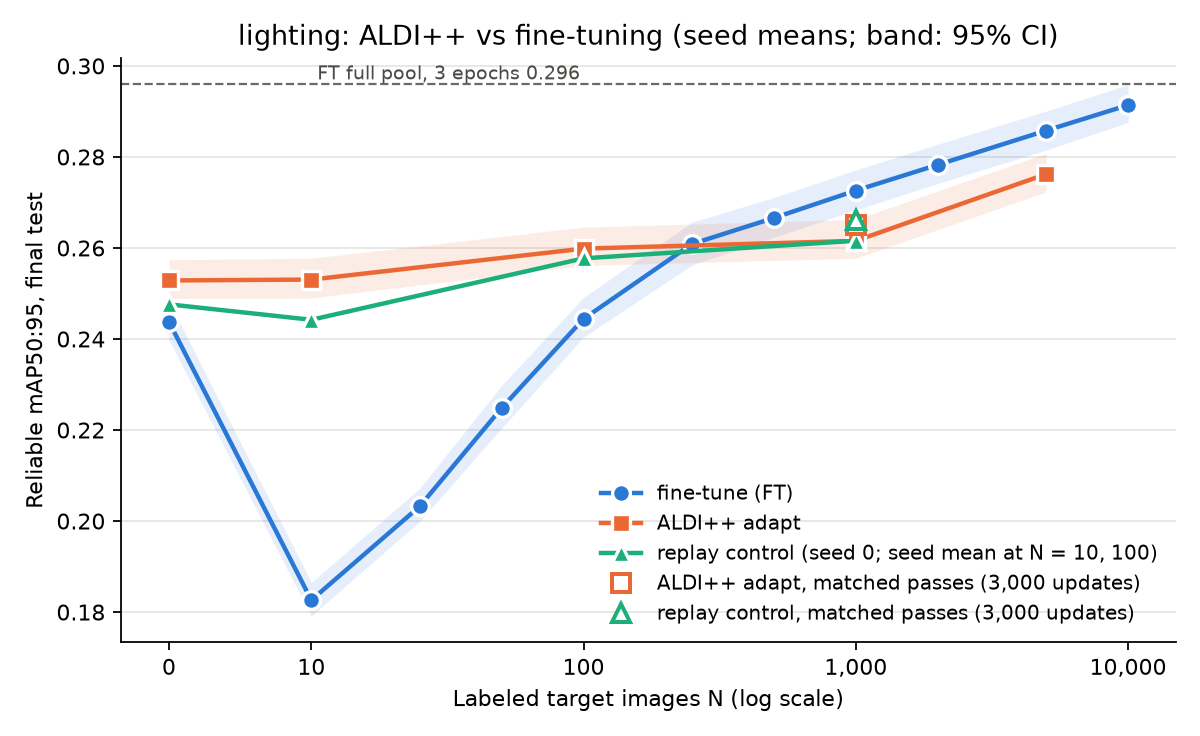
\includegraphics[width=\columnwidth]{rq5_lighting.png}
\caption{Lighting: FT, \aldi and the replay arm as a function of the budget $N$ (mean over seeds, 95\% CI bands). The open squares and triangles are the matched-passes experiment at $N = 1{,}000$ (3,000 updates).}
\label{fig:rq5-lighting}
\end{figure}

\begin{figure}[t]
\centering
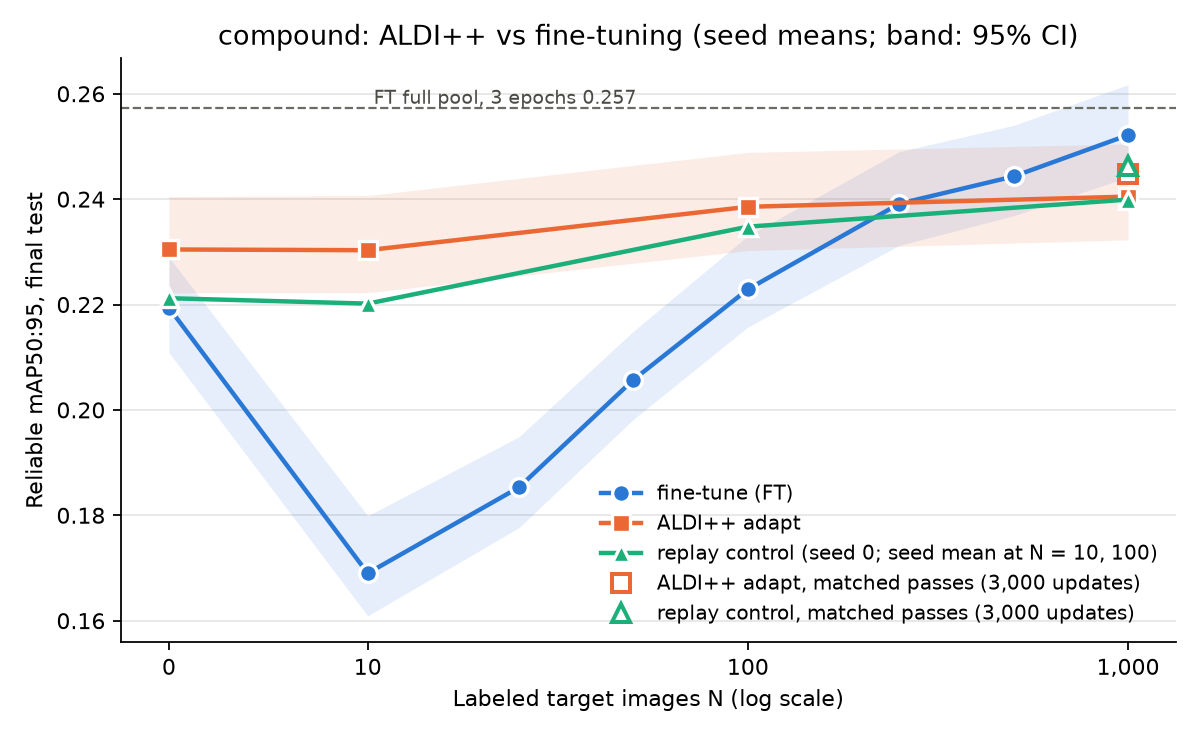
\includegraphics[width=\columnwidth]{rq5_compound.png}
\caption{Compound: same layout as Fig.~\ref{fig:rq5-lighting}.}
\label{fig:rq5-compound}
\end{figure}

\begin{figure}[t]
\centering
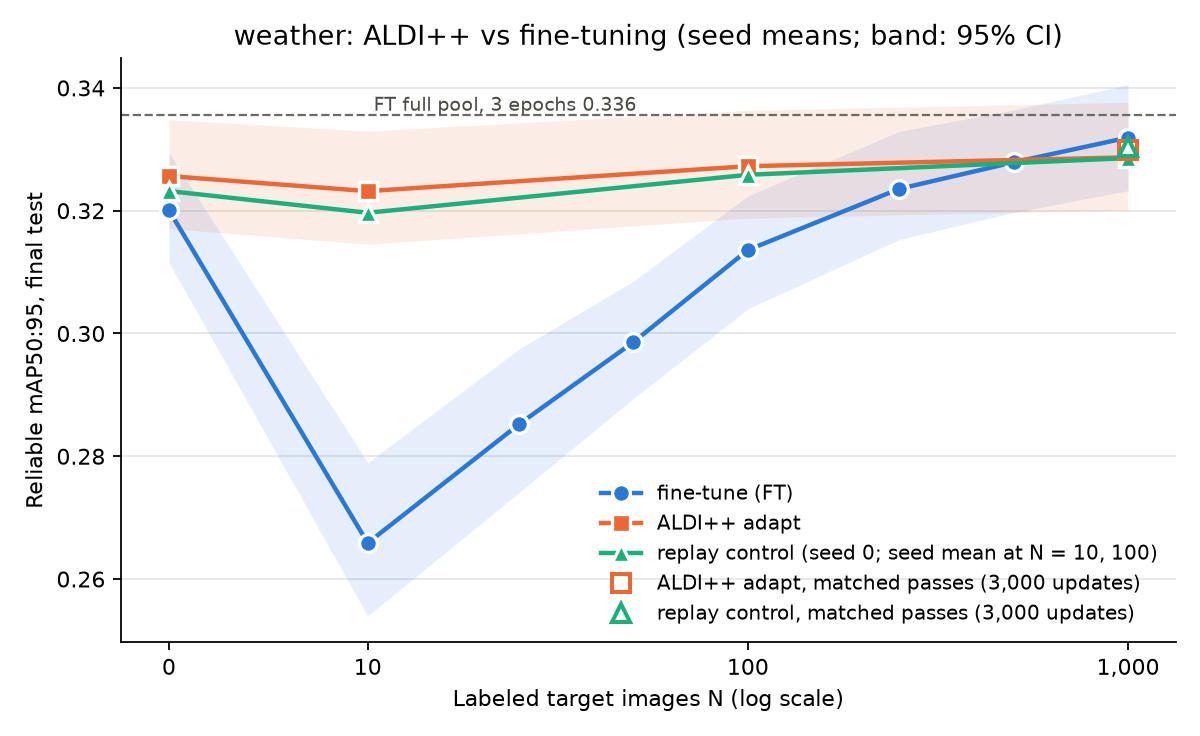
\includegraphics[width=\columnwidth]{rq5_weather.png}
\caption{Weather: same layout as Fig.~\ref{fig:rq5-lighting}. Note that the vertical-axis range is much narrower.}
\label{fig:rq5-weather}
\end{figure}

\subsection{Decomposition with the Replay Arm}\label{sec:decomp}

\begin{table}[t]
\centering
\caption{Replay share $=$ (replay $-$ FT) / (adapt $-$ FT): the part of \aldi's advantage over FT that the arm without adaptation reproduces (95\% CI).}
\label{tab:share}
\footnotesize
\setlength{\tabcolsep}{3pt}
\begin{tabular}{@{}>{\raggedright\arraybackslash}p{0.62in}>{\raggedright\arraybackslash}p{0.78in}>{\raggedright\arraybackslash}p{0.78in}>{\raggedright\arraybackslash}p{0.92in}@{}}
\toprule
$N$ & lighting & weather & compound \\
\midrule
10 (3 seeds) & \textbf{0.87} (0.85--0.90) & \textbf{0.94} (0.91--0.96) & \textbf{0.83} (0.80--0.86) \\
100 (3 seeds) & \textbf{0.86} (0.78--0.90) & \textbf{0.90} (0.81--1.04) & \textbf{0.76} (0.62--0.85) \\
1,000 (seed 0; deficit) & 1.05 (0.95--1.16) & undetermined (926/1,000) & 0.97 (0.82--1.15) \\
0 (seed 0; no labels) & 0.39 (0.28--0.45) & undetermined (287/1,000) & 0.17 ($-$0.04 to 0.35); 1/1,000 undetermined \\
\bottomrule
\end{tabular}
\tabnote{The number in parentheses after ``undetermined'' is the number of bootstrap resamples, out of 1,000, with $|\mathrm{adapt} - \mathrm{FT}| < 0.005$.}
\end{table}

\claimbox{\textbf{Main claim.} At $N = 10$ and $N = 100$, the replay arm reproduces 76--94\% of \aldi's advantage over FT in all three shifts. \aldi is genuinely ahead of FT in all six cells, every lower CI bound is above 0.5, and in no cell are more than 5\% of the bootstrap resamples undetermined. The condition recorded in advance for stating the claim is met at both budgets.\par\smallskip
Statement: \textbf{at small labeled budgets, most of the advantage of domain adaptation over fine-tuning is not adaptation.} The claim applies only to the two budgets tested ($N = 10$, $N = 100$), only to the advantage \emph{over fine-tuning}, and is not stated for $N = 0$.}

At $N = 1{,}000$, adapt $-$ FT is negative, so the share in the $N = 1{,}000$ row of Table~\ref{tab:share} says that the \emph{deficit} lies almost entirely in replay; this is not evidence for the main claim. At $N = 0$ the opposite holds: for lighting and compound, most of the gain comes from distillation, so the claim is not stated for the unlabeled case.

FT at $N \leq 50$ is below even the source model, so the same numbers read differently when the baseline is ``no fine-tuning''. Table~\ref{tab:vssource} recomputes the decomposition with the source model as the baseline.

\begin{table}[t]
\centering
\caption{Gain over the source model (mAP $-$ zero-shot). FT: mean of 3 seeds; replay and \aldi: 3 seeds at $N = 10$ and 100, seed 0 at $N = 1{,}000$ (original number of updates).}
\label{tab:vssource}
\footnotesize
\setlength{\tabcolsep}{3pt}
\begin{tabular}{@{}lrccc>{\raggedright\arraybackslash}p{1.2in}@{}}
\toprule
Shift & $N$ & FT & replay & \aldi & replay / \aldi (95\% CI) \\
\midrule
lighting & 10 & $-$0.061 & 0.000 & +0.009 & 0.05 ($-$0.09 to 0.21) \\
 & 100 & +0.001 & +0.014 & +0.016 & 0.87 (0.80--0.91) \\
 & 1,000 & +0.029 & +0.018 & +0.018 & 0.97 (0.92--1.03) \\
\addlinespace[2pt]
weather & 10 & $-$0.054 & 0.000 & +0.003 & undetermined (908/1,000) \\
 & 100 & $-$0.007 & +0.006 & +0.007 & 0.80 (0.57--1.07); 29/1,000 undetermined \\
 & 1,000 & +0.012 & +0.008 & +0.008 & 1.00 (0.86--1.24); 1/1,000 undetermined \\
\addlinespace[2pt]
compound & 10 & $-$0.050 & +0.001 & +0.011 & 0.07 ($-$0.22 to 0.29) \\
 & 100 & +0.003 & +0.015 & +0.019 & 0.80 (0.72--0.88) \\
 & 1,000 & +0.033 & +0.021 & +0.020 & 1.02 (0.92--1.12) \\
\bottomrule
\end{tabular}
\end{table}

Tables~\ref{tab:share}, \ref{tab:vssource} and~\ref{tab:cells} (the per-cell decomposition) support four conclusions:
\begin{enumerate}
\item \textbf{At $N = 10$, \aldi's large advantage over FT is damage that FT does to itself, not adaptation.} FT with 10 images and 500 updates makes the model 0.05--0.06 AP worse than the source model. Replay only has to avoid that damage to reproduce 83--94\% of the advantage. Against the source model, replay gains nothing (all CIs contain 0), and \aldi gains only +0.003 to +0.011 AP, no more than it gains with no labels at all (+0.006 to +0.011 at $N = 0$). In other words, the 10 labeled images add nothing; the small remaining gain comes from distillation.
\item \textbf{At $N = 100$, the two baselines give the same conclusion; this is the cleanest evidence.} FT is now roughly equal to the source model on lighting (+0.001) and compound (+0.003), with CIs that contain 0. On weather, FT is still 0.007 AP below the source model (CI $-0.012$ to $-0.002$), so part of the advantage here is still FT's damage. Replay reproduces 76--90\% of the advantage over FT and 80--87\% of the gain over the source model.
\item \textbf{Distillation on unlabeled images has a real but small value:} about 0.003--0.010 AP when $N \leq 10$, $\leq 0.004$ AP at $N = 100$ (on weather, the 3-seed mean is +0.001 with a CI that contains 0), and it falls to 0 at $N = 1{,}000$.
\item \textbf{The deficit at $N = 1{,}000$ is not caused by distillation.} Replay trails FT by almost the same amount, and against the source model replay equals \aldi (ratio $\approx 1$). The matched-passes experiment in Section~\ref{sec:matched} gives the same conclusion.
\end{enumerate}

\begin{table}[t]
\centering
\caption{Per-cell decomposition, seed 0 (original number of updates). The CIs reflect test-image noise only.}
\label{tab:cells}
\footnotesize
\setlength{\tabcolsep}{3pt}
\begin{tabular}{@{}lrll@{}}
\toprule
Shift & $N$ & adapt $-$ replay & replay $-$ FT \\
\midrule
lighting & 0 & +0.006 & +0.004 \\
 & 10 & +0.009 & +0.062 \\
 & 100 & +0.002 & +0.012 \\
 & 1,000 & 0.000 (CI contains 0) & $-$0.010 \\
\addlinespace[2pt]
weather & 0 & +0.003 & +0.003 \\
 & 10 & +0.004 & +0.064 \\
 & 100 & +0.003 & +0.016 \\
 & 1,000 & 0.000 (CI contains 0) & $-$0.003 \\
\addlinespace[2pt]
compound & 0 & +0.009 & +0.002 (CI contains 0) \\
 & 10 & +0.010 & +0.046 \\
 & 100 & +0.004 & +0.013 \\
 & 1,000 & 0.000 (CI contains 0) & $-$0.012 \\
\bottomrule
\end{tabular}
\tabnote{At $N = 0$, ``replay'' is the source model trained further on source images with strong augmentation and EMA, so replay $-$ FT here is replay $-$ zero-shot.}
\end{table}

\subsection{Matched-Passes Experiment at \texorpdfstring{$N = 1{,}000$}{N = 1,000}}\label{sec:matched}

In the original grid, at $N = 1{,}000$, FT runs 1,500 updates with 2 labeled target images per step (about 3,000 passes), while \aldi and replay run 2,000 updates with 1 labeled target image per step (about 2,000 passes). \aldi's deficit is therefore confounded with the difference in the amount of labeled training. The matched-passes experiment reruns \aldi and replay with 3,000 updates and 3 seeds. The reading rule, recorded before scoring: ``FT leads from $N = 1{,}000$'' stands when the difference is $\leq -0.005$ and the upper CI bound is below 0; otherwise it is withdrawn. The text of the rule does not say whether it applies to the three shifts pooled or to each shift separately; here it is applied per shift, and this way of applying it was recorded after scoring.

\begin{table*}[t]
\centering
\caption{$N = 1{,}000$ with matched labeled target-image passes (3,000 updates, 3 seeds; 95\% CI).}
\label{tab:matched}
\footnotesize
\setlength{\tabcolsep}{3pt}
\begin{tabular}{@{}lcccc>{\raggedright\arraybackslash}p{1.2in}@{}}
\toprule
Shift & \begin{tabular}[b]{@{}c@{}}original\\\aldi $-$ FT\end{tabular} & \begin{tabular}[b]{@{}c@{}}matched\\\aldi $-$ FT\end{tabular} & \begin{tabular}[b]{@{}c@{}}matched\\replay $-$ FT\end{tabular} & \begin{tabular}[b]{@{}c@{}}\aldi $-$ replay\\(matched)\end{tabular} & Verdict under the rule \\
\midrule
lighting & $-$0.0111 & $-$0.0076 & $-$0.0064 & $-$0.0012 & ``FT leads'' stands \\
 & & ($-$0.0091, $-$0.0058) & ($-$0.0077, $-$0.0049) & ($-$0.0021, $-$0.0002) & \\
\addlinespace[2pt]
weather & $-$0.0032 & $-$0.0021 & $-$0.0015 & $-$0.0005 & withdrawn: no meaningful difference \\
 & & ($-$0.0038, +0.0002) & ($-$0.0034, +0.0006) & ($-$0.0022, +0.0011) & \\
\addlinespace[2pt]
compound & $-$0.0117 & $-$0.0074 & $-$0.0058 & $-$0.0016 & ``FT leads'' stands \\
 & & ($-$0.0097, $-$0.0047) & ($-$0.0082, $-$0.0035) & ($-$0.0035, +0.0007) & \\
\bottomrule
\end{tabular}
\end{table*}

\begin{itemize}
\item The extra 1,000 updates (Table~\ref{tab:matched}) give \aldi +0.0034 / +0.0012 / +0.0043 AP (lighting / weather / compound), closing about a third of the gap (31\% / 36\% / 36\%), but they do not eliminate it on lighting and compound.
\item \textbf{Distillation contributes nothing to reliable mAP at $N = 1{,}000$.} After matching, \aldi is level with or slightly below replay; on lighting the CI of the difference does not contain 0. Per class, the changes offset each other: car gains +0.003 (lighting) and +0.002 (compound), while traffic light and traffic sign on lighting drop by 0.004 and 0.005.
\item Against the source model, replay reproduces all of \aldi's gain after matching: ratios of 1.06 (1.01--1.10) / 1.05 (0.89--1.26) / 1.06 (0.98--1.15).
\item The crossover \Nx under the original rule is unchanged, $(100, 1{,}000]$ in all three shifts. On weather it says only that \aldi's advantage disappears, not that FT pulls ahead.
\item \textbf{Limit of the matching:} it matches the number of labeled image passes that the \emph{student} sees, but the model that is scored is the EMA teacher. After 3,000 updates the source-model initialization still carries a weight of $0.9996^{3000} \approx 0.30$ in the teacher (0.45 after 2,000 updates). This lag is an alternative explanation for the remaining deficit.
\end{itemize}

\subsection{Equivalent Labeled Budget}\label{sec:neq}

\begin{table}[t]
\centering
\caption{\Neq: the number of images FT needs to reach the same mAP as \aldi (original number of updates; 95\% CI).}
\label{tab:neq}
\footnotesize
\setlength{\tabcolsep}{3pt}
\begin{tabular}{@{}lccccc@{}}
\toprule
 & \multicolumn{5}{c}{DA} \\
\cmidrule(l){2-6}
Shift & $N = 0$ & $N = 10$ & $N = 100$ & $N = 1{,}000$ & $N = 5{,}000$ \\
\midrule
lighting & 160 & 162 & 236 & 272 & 1,556 \\
 & (142--184) & (145--183) & (215--287) & (235--344) & (1,343--1,894) \\
\addlinespace[2pt]
weather & 349 & 242 & 451 & 575 & \\
 & (240--511) & (184--379) & (313--672) & (413--834) & \\
\addlinespace[2pt]
compound & 153 & 152 & 242 & 300 & \\
 & (123--182) & (121--180) & (209--332) & (233--410) & \\
\bottomrule
\end{tabular}
\end{table}

\begin{itemize}
\item Unlabeled \aldi (unsupervised domain adaptation, UDA) is worth about \textbf{150--350 labeled images} when FT is used with this schedule (Table~\ref{tab:neq}).
\item \aldi with 10 labeled images is no better than unlabeled \aldi: those 10 images add almost nothing.
\item With the original number of updates, \aldi with 1,000 labeled images is equivalent to FT with only 270--575 images. This figure is confounded with the difference in the number of labeled image passes and is not recomputed for the matched-passes experiment; on weather, no meaningful difference remains after matching, so the figure of 575 is not to be read as \aldi losing to FT.
\end{itemize}

\subsection{Weather: The Third Replication of the Decomposition}\label{sec:weather-rep}

The weather shift leaves very little to recover (Section~\ref{sec:drop}), so its thresholds can hardly be measured. The decomposition, however, needs no recovery denominator, and weather shows the same pattern as the other two shifts: a replay share of 0.94 at $N = 10$ and 0.90 at $N = 100$, with lower CI bounds above 0.5; distillation contributes only +0.001 AP at $N = 100$ (3-seed mean, CI contains 0); and at $N = 1{,}000$, after matching, neither \aldi nor replay differs meaningfully from FT. Every weather $\Delta$ except the one at $N = 10$ is small in absolute AP ($|\Delta| \leq 0.014$). The role of weather in this paper is therefore that of the third replication of the decomposition, not a third threshold measurement.

% Sections 6 and 7: data-efficiency curves (context) and labeled-budget thresholds (secondary result).

\section{Context: Data-Efficiency Curves}\label{sec:curves}

\subsection{How Much Domain Shift Reduces mAP (RQ1)}\label{sec:drop}

\begin{table*}[t]
\centering
\caption{Zero-shot drop relative to the source model on the source test set (0.342), and the gap remaining after the ceiling.}
\label{tab:drop}
\footnotesize
\setlength{\tabcolsep}{3pt}
\begin{tabular}{@{}lccccccc@{}}
\toprule
Shift & \mAPzero & Drop (95\% CI) & Relative drop & 3-epoch ceiling & Remaining gap & 12-epoch ceiling & Remaining gap \\
\midrule
lighting & 0.244 & 0.098 (0.092--0.106) & 28.8\% & 0.296 & 0.046 & 0.299 & 0.043 \\
weather  & 0.320 & 0.022 (0.012--0.032) & 6.5\%  & 0.336 & 0.007 & 0.331 & 0.011 \\
compound & 0.219 & 0.123 (0.112--0.133) & 35.9\% & 0.257 & 0.085 & 0.258 & 0.084 \\
\bottomrule
\end{tabular}
\tabnote{Remaining gap $= \mAPsrc - \text{ceiling}$. Ceilings are means over 2 seeds.}
\end{table*}

Table~\ref{tab:drop} gives the zero-shot drop of each shift and the gap that remains after each ceiling.

\textbf{Interaction.} $\mathrm{Drop}(\text{compound}) - \mathrm{Drop}(\text{lighting}) - \mathrm{Drop}(\text{weather}) = +0.002$ AP (CI $-0.012$ to $+0.016$). The point estimate is close to 0, but the test is weak: the CI half-width is 0.014 AP, equal to 63\% of the entire weather effect (0.022 AP); the smallest interaction detectable with 80\% power is 0.020 AP, that is, 91\% of the weather effect. The correct conclusion is: \textbf{these data cannot detect an interaction smaller than about 0.014--0.020 AP.} This is not evidence that the compound shift is additive.

\begin{table}[t]
\centering
\caption{Denominator of recovery (ceiling $-$ zero-shot).}
\label{tab:denom}
\footnotesize
\setlength{\tabcolsep}{3pt}
\begin{tabular}{@{}lcccc@{}}
\toprule
 & \multicolumn{2}{c}{3-epoch ceiling} & \multicolumn{2}{c}{12-epoch ceiling} \\
\cmidrule(lr){2-3}\cmidrule(lr){4-5}
Shift & Denominator & Multiple & Denominator & Multiple \\
 & (95\% CI) & of 0.01 & (95\% CI) & of 0.01 \\
\midrule
lighting & 0.052 (0.050--0.054) & 5.2 & 0.055 (0.053--0.058) & 5.5 \\
compound & 0.038 (0.034--0.042) & 3.8 & 0.038 (0.034--0.043) & 3.8 \\
weather  & 0.015 (0.012--0.018) & 1.5 & 0.011 (0.007--0.014) & 1.1 \\
\bottomrule
\end{tabular}
\end{table}

The weather denominator (Table~\ref{tab:denom}) is only one and a half times the minimum with the 3-epoch ceiling and sits close to the minimum with the 12-epoch ceiling. Per class (3-epoch ceiling): pedestrian 0.022, car 0.018, traffic light 0.013, traffic sign 0.009, so traffic sign is already below the minimum. In 1,000 bootstrap resamples, the denominator falls below the minimum 115 times for traffic light and 713 times for traffic sign.

\subsection{Recovery Curves (RQ2)}\label{sec:recovery}

\begin{table*}[t]
\centering
\caption{Recovery of reliable mAP against the 3-epoch ceiling (mean of 3 seeds, 95\% hierarchical bootstrap CI).}
\label{tab:recovery}
\footnotesize
\setlength{\tabcolsep}{3pt}
\begin{tabular}{@{}lccc@{}}
\toprule
$N$ & lighting & weather & compound \\
\midrule
10     & $-$1.17 ($-$1.23, $-$1.10) & $-$3.51 ($-$4.67, $-$2.71) & $-$1.33 ($-$1.59, $-$1.07) \\
25     & $-$0.78 ($-$0.83, $-$0.72) & $-$2.26 ($-$3.12, $-$1.60) & $-$0.90 ($-$1.11, $-$0.71) \\
50     & $-$0.36 ($-$0.43, $-$0.29) & $-$1.39 ($-$2.01, $-$0.96) & $-$0.36 ($-$0.49, $-$0.22) \\
100    & 0.01 ($-$0.03, 0.05)       & $-$0.42 ($-$0.85, $-$0.10) & 0.09 ($-$0.01, 0.20) \\
250    & 0.33 (0.28, 0.36)          & 0.22 (0.05, 0.35)          & 0.52 (0.46, 0.58) \\
500    & 0.44 (0.41, 0.46)          & 0.50 (0.39, 0.60)          & 0.66 (0.61, 0.71) \\
1,000  & 0.55 (0.52, 0.57)          & 0.77 (0.66, 0.86)          & 0.87 (0.82, 0.91) \\
2,000  & 0.66 (0.63, 0.69)          &                            & \\
5,000  & 0.80 (0.78, 0.82)          &                            & \\
10,000 & 0.91 (0.89, 0.93)          &                            & \\
full pool & 1 (18,015 images)       & 1 (1,985 images)           & 1 (1,738 images) \\
\bottomrule
\end{tabular}
\end{table*}

\textbf{At small $N$, fine-tuning makes the model worse than zero-shot.} Recovery is negative at $N \leq 50$ in all three shifts, and at $N = 100$ for weather (Table~\ref{tab:recovery}, Fig.~\ref{fig:rec-lighting}). The cause is the fixed schedule: 10 images receive 500 updates, that is, about 100 epochs. This is exactly the region where \aldi has its largest advantage, and Section~\ref{sec:decomp} shows that most of that advantage is due to FT overfitting. At large $N$, source forgetting also rises again (Section~\ref{sec:secondary}).

\begin{figure}[t]
\centering
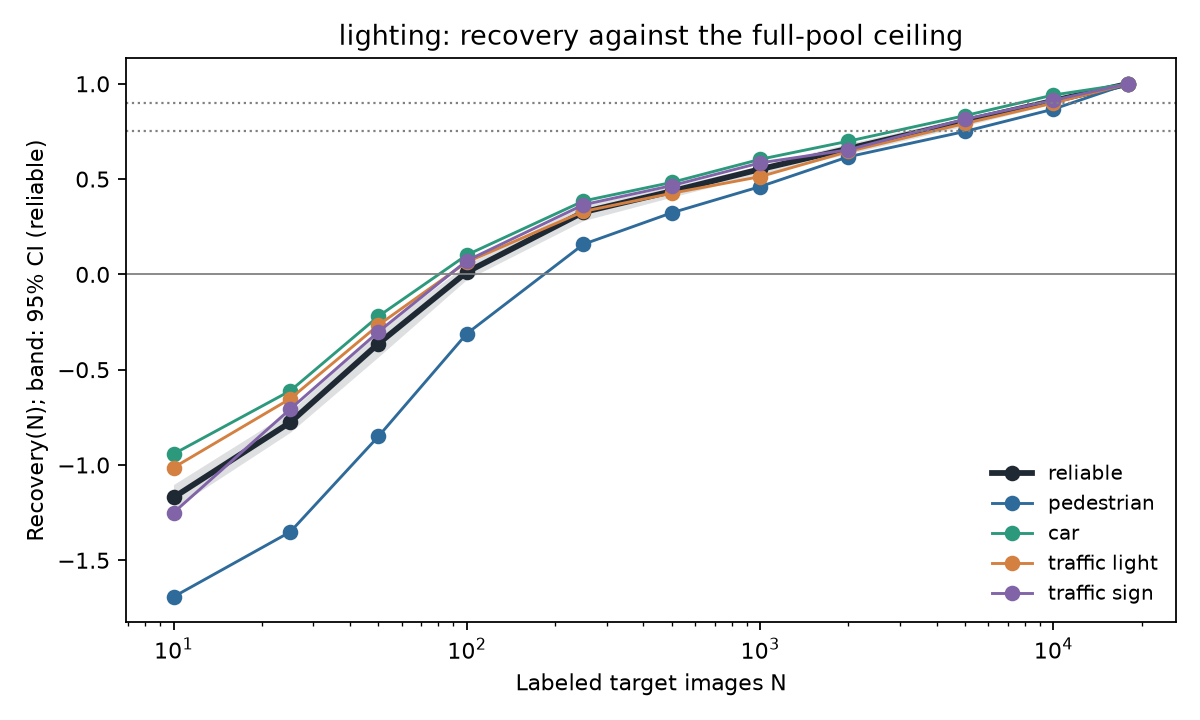
\includegraphics[width=\columnwidth]{recovery_lighting.png}
\caption{Lighting: recovery against the 3-epoch ceiling (mean of 3 seeds), for reliable mAP and for each class; the gray band is the 95\% CI of reliable mAP. The two dotted lines mark the 0.75 and 0.90 levels.}
\label{fig:rec-lighting}
\end{figure}

\begin{table}[t]
\centering
\caption{Per-class recovery at $N = 1{,}000$, 3-epoch ceiling.}
\label{tab:perclass}
\footnotesize
\setlength{\tabcolsep}{3pt}
\begin{tabular}{@{}lcccc@{}}
\toprule
Shift & pedestrian & car & traffic light & traffic sign \\
\midrule
lighting & 0.46 & 0.60 & 0.51 & 0.58 \\
weather  & 0.82 & 0.82 & \begin{tabular}[t]{@{}c@{}}undetermined\\(105/1,000)\end{tabular} & undetermined \\
compound & \begin{tabular}[t]{@{}c@{}}undetermined\\(120/1,000)\end{tabular} & 0.88 & 0.88 & 0.82 \\
\bottomrule
\end{tabular}
\end{table}

On lighting, against the 3-epoch ceiling, pedestrian recovers slowest (0.46; Table~\ref{tab:perclass}). Against the 12-epoch ceiling, traffic light is slowest (0.44) and pedestrian reaches 0.54 (0.40, 0.69), because 12 epochs raise the traffic light ceiling and lower the pedestrian ceiling. The ordering of the classes therefore depends on the ceiling, and it is not enough to separate re-learning the class distribution from learning new visual features. On compound and weather, the classes that can still be cited track each other closely.

\subsection{12-Epoch versus 3-Epoch Ceiling}\label{sec:ceiling12}

If the 3-epoch ceiling were undertrained, the recovery denominator would be small, recovery would be inflated, and every threshold would be a lower bound on the true requirement. The 12-epoch ceiling was run to test this. The rule, written before scoring: the 12-epoch ceiling replaces the 3-epoch ceiling as the denominator \textbf{regardless of the outcome}; ``materially higher'' means a paired difference $\geq 0.005$ AP with the lower CI bound above 0; both threshold tables are reported.

\begin{table*}[t]
\centering
\caption{12-epoch versus 3-epoch ceiling (reliable mAP, mean of 2 seeds, paired difference).}
\label{tab:ceil}
\footnotesize
\setlength{\tabcolsep}{3pt}
\begin{tabular}{@{}llcccc@{}}
\toprule
Shift & Pool & 3-epoch ceiling & 12-epoch ceiling & 12 $-$ 3 epochs (95\% CI) & Materially higher? \\
\midrule
lighting & full pool (18,015) & 0.2960 & 0.2989 & $+$0.0029 ($+$0.0014, $+$0.0041) & no \\
lighting & 1,738              & 0.2777 & 0.2756 & $-$0.0021 ($-$0.0031, $-$0.0007) & no \\
weather  & full pool (1,985)  & 0.3355 & 0.3310 & $-$0.0045 ($-$0.0067, $-$0.0025) & no \\
weather  & 1,738              & 0.3344 & 0.3300 & $-$0.0044 ($-$0.0067, $-$0.0022) & no \\
compound & full pool (1,738)  & 0.2572 & 0.2578 & $+$0.0005 ($-$0.0021, $+$0.0037) & no \\
\bottomrule
\end{tabular}
\end{table*}

\begin{itemize}
\item \textbf{No ceiling is materially higher} (Table~\ref{tab:ceil}). On the lighting full pool, 12 epochs exceed 3 epochs by 0.003 AP: statistically significant, but below the preset level of 0.005.
\item \textbf{On the small pools, 12 epochs either do not help or make things worse.} Compound is unchanged; weather and the 1,738-image lighting pool drop by 0.0021--0.0045 AP. This is consistent with 12 epochs starting to overfit at this pool size, but it has not been verified, and compound (also 1,738 images) does not drop.
\item Per class, only traffic light ($+0.0077$) and traffic sign ($+0.0053$) on the lighting full pool are materially higher.
\item Source forgetting is heavier at 12 epochs: $-0.043$ / $-0.015$ / $-0.032$ AP on the source test set (lighting / weather / compound), against $-0.026$ / $-0.005$ / $-0.018$ for the 3-epoch ceiling.
\end{itemize}

Per the rule, \mAPc is the 12-epoch ceiling: 0.2989 / 0.3310 / 0.2578. With this ceiling, the 3-epoch full-pool run becomes the top rung of the ladder and is a measurement, no longer equal to 1 by definition (Table~\ref{tab:rec2}, Figs.~\ref{fig:rec-lighting-e12} and~\ref{fig:rec-compound-e12}). Both ceilings are presented side by side; neither is chosen as better after the results have been seen.

\begin{table*}[t]
\centering
\caption{Recovery against the two ceilings (seed mean, 95\% CI).}
\label{tab:rec2}
\footnotesize
\setlength{\tabcolsep}{3pt}
\begin{tabular}{@{}lcccc@{}}
\toprule
 & \multicolumn{2}{c}{lighting} & \multicolumn{2}{c}{compound} \\
\cmidrule(lr){2-3}\cmidrule(lr){4-5}
$N$ & 3-epoch ceiling & 12-epoch ceiling & 3-epoch ceiling & 12-epoch ceiling \\
\midrule
100    & 0.01 ($-$0.03, 0.05) & 0.01 ($-$0.02, 0.05) & 0.09 ($-$0.01, 0.20) & 0.09 ($-$0.01, 0.20) \\
250    & 0.33 (0.28, 0.36)    & 0.31 (0.27, 0.34)    & 0.52 (0.46, 0.58)    & 0.51 (0.44, 0.59) \\
500    & 0.44 (0.41, 0.46)    & 0.41 (0.38, 0.44)    & 0.66 (0.61, 0.71)    & 0.65 (0.58, 0.72) \\
1,000  & 0.55 (0.52, 0.57)    & 0.52 (0.50, 0.55)    & 0.87 (0.82, 0.91)    & 0.85 (0.78, 0.92) \\
2,000  & 0.66 (0.63, 0.69)    & 0.63 (0.60, 0.65)    &                      & \\
5,000  & 0.80 (0.78, 0.82)    & 0.76 (0.73, 0.79)    &                      & \\
10,000 & 0.91 (0.89, 0.93)    & 0.86 (0.84, 0.89)    &                      & \\
full pool, 3 epochs & 1 (by definition) & 0.95 (0.93, 0.97) & 1 (by definition) & 0.99 (0.91, 1.05) \\
\bottomrule
\end{tabular}
\end{table*}

\begin{figure}[t]
\centering
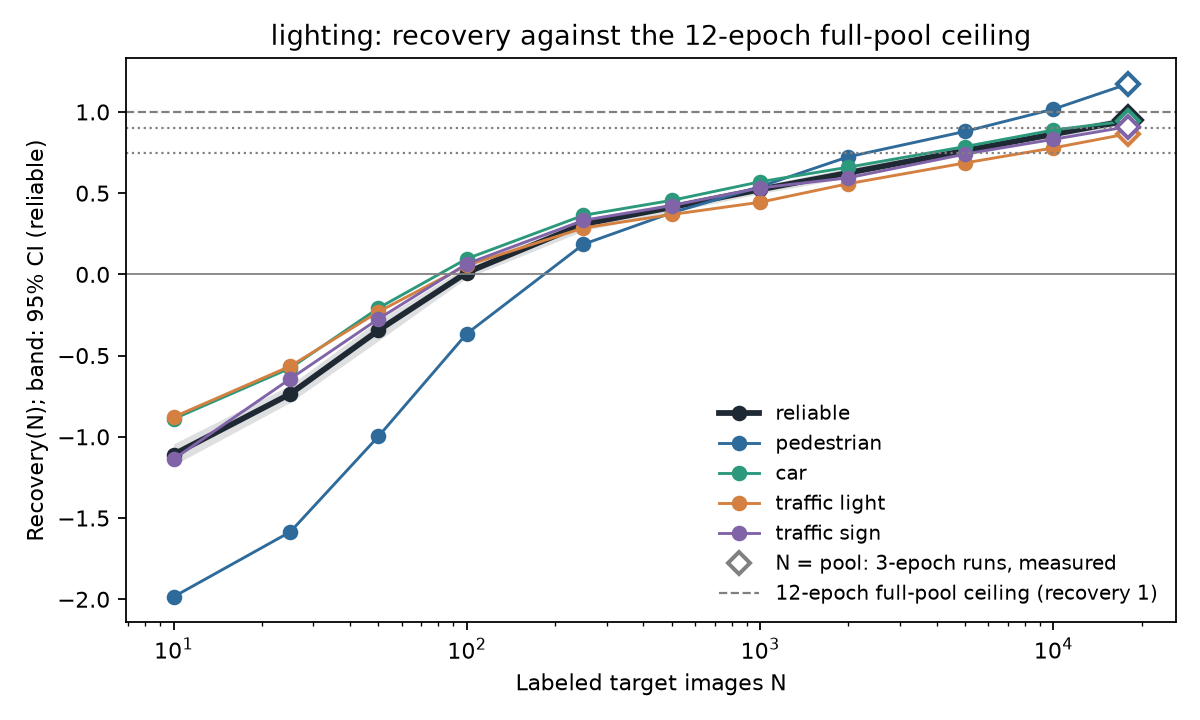
\includegraphics[width=\columnwidth]{recovery_lighting_e12.png}
\caption{Lighting: recovery against the 12-epoch ceiling. The last rung is the 3-epoch full-pool run, now a measurement (0.95).}
\label{fig:rec-lighting-e12}
\end{figure}

\begin{figure}[t]
\centering
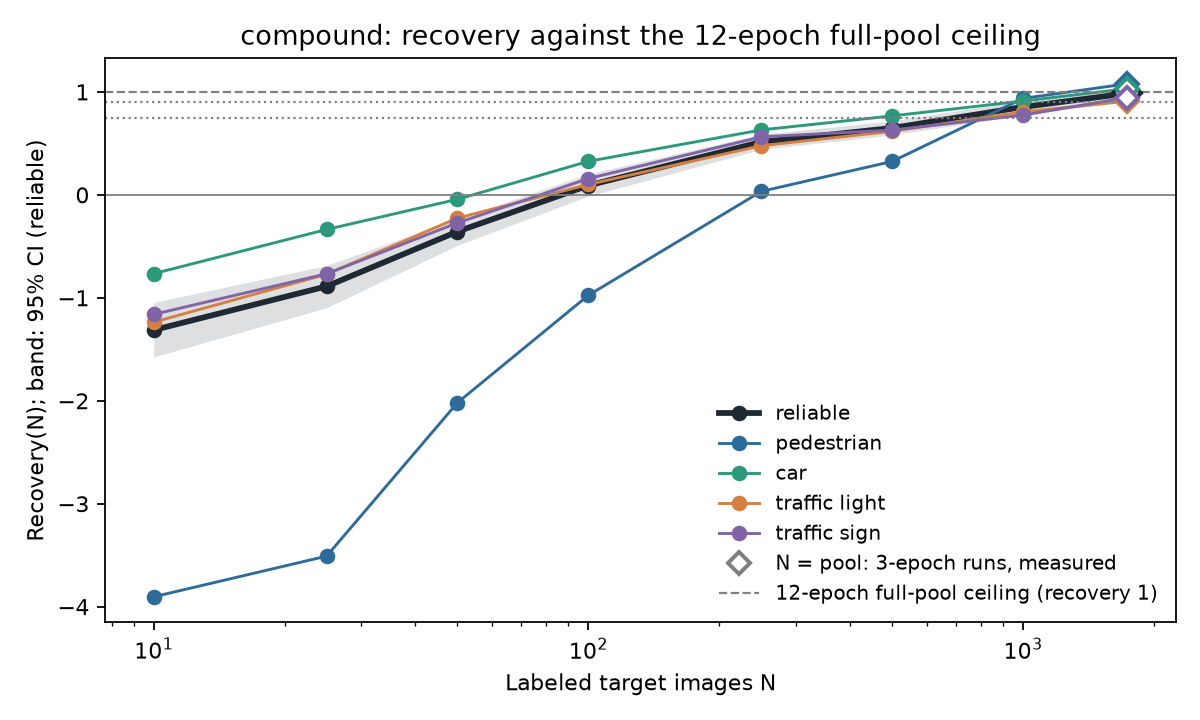
\includegraphics[width=\columnwidth]{recovery_compound_e12.png}
\caption{Compound: recovery against the 12-epoch ceiling. The last rung is the 3-epoch full-pool run (0.99).}
\label{fig:rec-compound-e12}
\end{figure}

Conclusion: \textbf{the 3-epoch ceiling is not materially undertrained relative to a schedule four times longer.} Twelve epochs add only 0.003 AP on the largest pool and nothing on the small pools. Note that the 12-epoch lighting ceiling, about 216,000 image passes, is still much shorter than the standard 1$\times$ schedule; this test rules out undertraining within the range of 3 to 12 epochs at the locked LR, but it does not rule out every possibility.

\section{Secondary Practical Result: Labeled-Budget Thresholds}\label{sec:thresholds}

\subsection{Thresholds against the Two Ceilings (RQ3)}\label{sec:thr-two}

\begin{table*}[t]
\centering
\caption{Thresholds \NBE, \Nsf, \Nnf (reliable mAP, full pool).}
\label{tab:thr}
\footnotesize
\setlength{\tabcolsep}{3pt}
\begin{tabular}{@{}llll@{}}
\toprule
Shift & Threshold & 3-epoch ceiling (CI range) & 12-epoch ceiling (CI range) \\
\midrule
lighting & \NBE & 100 (100--250) & 100 (100--250) \\
         & \Nsf & 5,000 (5,000) & 5,000 (5,000--10,000) \\
         & \Nnf & 10,000 (10,000--full pool) & full pool, 18,015 \\
\midrule
compound & \NBE & 100 (100--250) & 100 \\
         & \Nsf & 1,000 (1,000) & 1,000 \\
         & \Nnf & not determined within the pool ($>1{,}000$) & 1,738 (1,000--1,738) \\
\midrule
weather  & \NBE & 250 (250) & undetermined \\
         & \Nsf & 1,000 (1,000--full pool) & undetermined \\
         & \Nnf & not determined within the pool ($>1{,}000$) & undetermined \\
\bottomrule
\end{tabular}
\tabnote{With the 12-epoch ceiling, the ``full pool'' rung is the 3-epoch full-pool run, a real measurement. Each threshold is specific to the schedule $S = 500$, $E = 3$; it is not a property of the data alone.}
\end{table*}

\begin{itemize}
\item \textbf{Lighting:} \NBE is unchanged (Table~\ref{tab:thr}). \Nsf stays at the 5,000 rung, but only narrowly against the 12-epoch ceiling (recovery 0.76, CI 0.73--0.79). \Nnf moves from 10,000 up to the full pool, because recovery at $N = 10{,}000$ falls from 0.91 to 0.86.
\item \textbf{Compound:} \NBE and \Nsf are unchanged. \Nnf was previously not determined within the pool; with the 12-epoch ceiling, the 3-epoch full-pool rung reaches a recovery of 0.99, so $\Nnf = 1{,}738$.
\item \textbf{Weather is undetermined against the 12-epoch ceiling:} the denominator is only 0.011 AP, and 339 of the 1,000 bootstrap resamples of the recovery curve are undetermined. The 3-epoch full-pool run is even 0.0045 AP above the 12-epoch ceiling.
\item \textbf{Why \Nnf for weather and compound is not determined within the pool against the 3-epoch ceiling:} the largest rung actually measured is $N = 1{,}000$ (recovery 0.77 and 0.87); the next rung is the ceiling itself, equal to 1 by definition. The data only show that $\Nnf > 1{,}000$.
\item Three thresholds should be read with caution: weather $\Nsf = 1{,}000$ (recovery 0.77, lower CI bound 0.66); lighting $\Nnf = 10{,}000$ against the 3-epoch ceiling (lower CI bound 0.895); lighting $\NBE = 100$ (recovery $+0.01$, CI contains 0, a narrow break-even).
\end{itemize}

\subsection{Log-Linear Fit on the Positive Region}\label{sec:fit}

The fit is used only to interpolate between rungs. With the 3-epoch ceiling, all three shifts have a positive region starting at $N = 250$, but only lighting has at least 4 rungs (250--10,000, 6 rungs). With the 12-epoch ceiling, the 3-epoch full-pool rung belongs to the fit region, so compound reaches 4 rungs. The weather fit against the 12-epoch ceiling is not cited.

\begin{table*}[t]
\centering
\caption{Fit of $\mathrm{Recovery} = \alpha + \beta \cdot \ln N$ on the positive, monotonic region.}
\label{tab:fit}
\footnotesize
\setlength{\tabcolsep}{3pt}
\begin{tabular}{@{}lllccc@{}}
\toprule
Shift & Ceiling & Fit region & $R^2$ & \Nsf from fit (95\% CI) & \Nnf from fit (95\% CI) \\
\midrule
lighting & 3 epochs  & 250--10,000, 6 rungs & 0.9999 & 3,570 (3,250--3,960) & 9,200 (8,280 to $>10{,}000$) \\
lighting & 12 epochs & 250--18,015, 7 rungs & 0.9999 & 4,690 (4,070--5,340) & 12,800 (10,870--14,970) \\
compound & 12 epochs & 250--1,738, 4 rungs  & 0.9937 & 680 (530--880)       & 1,240 (980--1,630) \\
\bottomrule
\end{tabular}
\end{table*}

\begin{itemize}
\item Lighting (Table~\ref{tab:fit}): \Nsf lies in the range 3,570--4,690 images and \Nnf in the range 9,200--12,800 images, depending on the ceiling. The threshold against the 3-epoch ceiling is a lower bound and the one against the 12-epoch ceiling is an upper bound, because the large rungs of the ladder are trained for only 3 epochs. Both fall within the corresponding ladder interval; the ladder interval remains the main result.
\item A high $R^2$ on the fit region is not strong evidence, because the region has only 4--7 points that are nearly collinear in $\ln N$. A more meaningful test is a held-out check: a fit on the three lighting rungs 250, 500 and 1,000 predicts 0.663 / 0.812 / 0.924 at $N = 2{,}000$ / $5{,}000$ / $10{,}000$, against measured values of 0.660 / 0.804 / 0.911 (3-epoch ceiling). The error grows with $N$ ($+0.003$, $+0.008$, $+0.013$), so the fit is slightly optimistic when extrapolating.
\item Sensitivity to the choice of region: if the region starts at the point estimate of \NBE ($N = 100$), the lighting $R^2$ drops to 0.973 with the 3-epoch ceiling; the $N = 100$ rung is not yet in the log-linear region.
\item The full-pool point lies almost exactly on the log-linear line of the smaller rungs (predicted 1.007 against the 3-epoch ceiling): according to the data, the lighting curve has not saturated.
\end{itemize}

\subsection{Weather in Raw AP}\label{sec:weather-raw}

Table~\ref{tab:weatherap} gives the weather reliable mAP at each rung and its change from zero-shot.

\begin{table}[t]
\centering
\caption{Weather: reliable mAP by $N$ (seed mean; zero-shot 0.3201).}
\label{tab:weatherap}
\footnotesize
\setlength{\tabcolsep}{3pt}
\begin{tabular}{@{}lcl@{}}
\toprule
$N$ & mAP & vs.\ zero-shot (95\% CI) \\
\midrule
10    & 0.2659 & $-$0.0542 ($-$0.0641, $-$0.0443) \\
25    & 0.2852 & $-$0.0349 \\
50    & 0.2986 & $-$0.0215 \\
100   & 0.3136 & $-$0.0065 ($-$0.0118, $-$0.0017) \\
250   & 0.3236 & $+$0.0035 \\
500   & 0.3279 & $+$0.0078 \\
1,000 & 0.3319 & $+$0.0118 ($+$0.0088, $+$0.0142) \\
full pool, 3 epochs  & 0.3355 & $+$0.0154 \\
full pool, 12 epochs & 0.3310 & $+$0.0109 \\
\bottomrule
\end{tabular}
\tabnote{CIs are available only for the three rungs computed in the RQ5 analysis. The $N = 1{,}000$ rung is already on par with the 12-epoch ceiling.}
\end{table}

\subsection{Comparison across Shifts at the Same Pool Size (RQ4)}\label{sec:rq4}

\begin{table*}[t]
\centering
\caption{Pool of 1,738 images, 3-epoch ceiling (2 seeds per shift).}
\label{tab:rq4}
\footnotesize
\setlength{\tabcolsep}{3pt}
\begin{tabular}{@{}lcccl@{}}
\toprule
Shift & Recovery, $N = 500$ (95\% CI) & Recovery, $N = 1{,}000$ (95\% CI) & \Nsf & \Nnf \\
\midrule
lighting & 0.67 (0.63, 0.72) & 0.85 (0.81, 0.90) & 1,000 & not determined within the pool ($>1{,}000$) \\
weather  & 0.54 (0.42, 0.65) & 0.82 (0.71, 0.92) & 1,000 (1,000--1,738) & not determined within the pool ($>1{,}000$) \\
compound & 0.66 (0.61, 0.71) & 0.87 (0.82, 0.91) & 1,000 & not determined within the pool ($>1{,}000$) \\
\bottomrule
\end{tabular}
\end{table*}

At the same pool size (Table~\ref{tab:rq4}), lighting and compound recover at almost the same rate; weather is slower at $N = 500$ but catches up at $N = 1{,}000$, and all three have $\Nsf = 1{,}000$. The differences between shifts in Section~\ref{sec:thr-two} therefore come mainly from the magnitude of the ceiling and the pool size, not from the speed of learning. Against the 12-epoch ceiling on the 1,738-image pool: lighting has $\Nsf = \Nnf = 1{,}000$ (recovery 0.91, CI 0.84--0.97), compound has $\Nsf = 1{,}000$ and $\Nnf = 1{,}738$, and weather is undetermined (denominator 0.0099 AP).

% Sections 8--11: secondary results, discussion, limitations, conclusion.
% Input by main.tex; no preamble here.

\section{Side Results}\label{sec:secondary}

\subsection{Source Forgetting}\label{sec:forgetting}

\begin{table}[t]
\centering
\caption{Change in reliable mAP on the source test set relative to the source model (mean over seeds).}
\label{tab:forget}
\footnotesize
\setlength{\tabcolsep}{3pt}
\begin{tabular}{@{}lccccc@{}}
\toprule
 & \multicolumn{3}{c}{FT} & \aldi{} & replay \\
\cmidrule(lr){2-4}
$N$ & lighting & weather & compound & (3 shifts) & (3 shifts) \\
\midrule
10 & $-$0.055 & $-$0.058 & $-$0.055 & $-$0.003 to $-$0.004 & $-$0.003 \\
100 & $-$0.019 & $-$0.018 & $-$0.022 & $-$0.001 to $-$0.002 & $\approx 0$ \\
1,000 & $-$0.012 & $-$0.006 & $-$0.016 & $\approx 0$ & $\approx 0$ \\
\begin{tabular}[t]{@{}l@{}}full pool,\\ 3 epochs\end{tabular} & $-$0.026 & $-$0.005 & $-$0.018 & & \\
\bottomrule
\end{tabular}
\end{table}

FT forgets the most at $N = 10$ (Table~\ref{tab:forget}). On lighting and compound, forgetting is smallest at $N = 250$ ($-0.011$ and $-0.014$) and then grows again at large $N$, because the number of updates grows. \aldi and replay show almost no forgetting, because they always mix source images into the batch; this is a practical advantage of the training recipe, and, again, not of adaptation. Lighting, $N = 5{,}000$: FT $-0.020$, \aldi $-0.010$. In the matched-passes experiment, \aldi changes by $-0.004$ / $-0.002$ / $-0.004$ AP and replay by 0.000 / $+0.001$ / 0.000.

\subsection{COCO-Initialization Control}\label{sec:coco}

\begin{table}[t]
\centering
\caption{Reliable mAP by initialization.}
\label{tab:coco}
\footnotesize
\setlength{\tabcolsep}{3pt}
\begin{tabular}{@{}lccc@{}}
\toprule
 & COCO & Source-model & \\
Shift, $N$ & initialization & initialization & Zero-shot \\
\midrule
lighting 100 / 1,000 & 0.171 / 0.220 & 0.244 / 0.273 & 0.244 \\
weather 100 / 1,000 & 0.209 / 0.267 & 0.314 / 0.332 & 0.320 \\
compound 100 / 1,000 & 0.149 / 0.198 & 0.223 / 0.252 & 0.219 \\
\bottomrule
\end{tabular}
\end{table}

Pretraining on the source domain accounts for most of the performance (Table~\ref{tab:coco}): with 1,000 target images, COCO initialization is still below zero-shot in all three shifts.

\section{Discussion}\label{sec:discussion}

\textbf{The advantage of DAOD also measures the weakness of the baseline.} At small budgets, the large advantage of \aldi over FT appears exactly where FT overfits: 10 images with 500 updates. An arm that keeps only the training recipe of \aldi (source-image mixing, strong augmentation, EMA), which is in essence a form of regularized fine-tuning, already obtains 76--94\% of \aldi's advantage over FT at $N = 10$ and $N = 100$. This result parallels the argument of ALDI: the reported advantage of DAOD depends on how the baseline is built. Here it is extended to the setting with target labels, and it is measured on all three shifts with the same conclusion.

\textbf{Genuine adaptation has value, but it is small and shrinks quickly.} Without labels, \aldi gains 0.006--0.011 AP over the source model, equivalent to about 150--350 labeled images under FT; distillation accounts for 0.003--0.009 AP of this (seed 0) and is most of the gain on lighting and compound. Once 100 labeled images are available, the contribution of distillation falls to $\leq 0.004$ AP; at 1,000 images it is 0.

\textbf{At $N = 1{,}000$, FT with the locked schedule leads} on lighting and compound, even when labeled image passes are matched; on lighting at $N = 5{,}000$, the conclusion is still confounded with the difference in image passes. The lag of the EMA teacher is an alternative explanation that has not been ruled out.

\textbf{Practical implications,} within the scope of this configuration:
\begin{itemize}
\item Below about 100 labeled images, fine-tuning with a fixed schedule is not advisable: it can make the model worse than no fine-tuning at all. The cheap part of \aldi (source-image mixing, strong augmentation, EMA) already gives most of the benefit, and it preserves performance on the source domain.
\item From about 1,000 labeled images on, fine-tuning matches or beats \aldi.
\item Reaching 75\% recovery takes about 5,000 images for lighting and 1,000 images for compound, under both ceilings.
\end{itemize}

\textbf{What must be tested to generalize these results:} an FT whose number of updates scales with $N$ (to determine whether avoiding overfitting is enough to erase the advantage at small $N$); other DAOD methods, each with its own replay arm on the same budgets; the matched-passes experiment at $N = 5{,}000$; rungs between 100 and 1,000 to locate the crossover; and a second detector.

\section{Limitations}\label{sec:limitations}

\begin{enumerate}
\item \textbf{One DAOD method, reimplemented.} \aldi was rewritten in torchvision with fixed $1280\times720$ images, no burn-in, a small batch and LR $10^{-3}$. The measured UDA gain is small ($+0.006$ to $+0.011$ AP). The main claim has so far been tested on only one method.
\item \textbf{One detector, one schedule.} Every threshold is specific to the schedule $S = 500$, $E = 3$; $E = 3$ was chosen by a margin of 0.0001 AP. With $E = 2$, every rung $N \geq 500$ would receive one third fewer updates.
\item \textbf{The small-$N$ advantage depends on the FT schedule.} FT uses a fixed 500 updates, so it overfits at $N \leq 50$; an FT whose number of updates scales with $N$ has not been run. The curves measure ``data plus the corresponding amount of training''.
\item \textbf{The matched-passes experiment was run only at $N = 1{,}000$,} and it matches only the student's image passes; the lag of the EMA teacher has not been separated out. On lighting at $N = 5{,}000$, the conclusion is still confounded with the difference in labeled image passes.
\item \textbf{The ceiling is a ceiling of the schedule.} The 12-epoch ceiling is still much shorter than the standard 1$\times$ schedule; the ladder rungs are trained for only 3 epochs, so the thresholds against the 12-epoch ceiling are upper bounds at the large rungs.
\item \textbf{Weather} has a denominator of 0.015 AP (3-epoch ceiling) and 0.011 AP (12-epoch ceiling); traffic sign is below the minimum. The weather thresholds against the 12-epoch ceiling are undetermined.
\item \textbf{The interaction test in RQ1 is weak:} it cannot detect an interaction smaller than about 0.014--0.020 AP.
\item \textbf{Some rules were set after the results had been seen} (Section~\ref{sec:rules}): the fit region, the 5\% rule for recovery, the side-by-side presentation of the two ceilings, and the sustained crossing for \Neq. The rule for the main claim was written after seed 0 had been seen; its independent confirmation comes from seeds 1 and 2 of the replay arm.
\item \textbf{The per-cell decomposition table uses only seed 0;} replay with the original number of updates at $N = 0$ and $N = 1{,}000$ has only seed 0.
\item \textbf{BDD100K labels from the 2018 release,} which has since been replaced by \texttt{det\_20}. Near-duplicate images and geographic dependence between splits have not been checked; the hashes rule out only exact duplicates.
\end{enumerate}

\section{Conclusion}\label{sec:conclusion}

At small labeled budgets ($N = 10$ and $N = 100$), a control arm without adaptation reproduces 76--94\% of \aldi's advantage over fine-tuning, in all three shifts and with 3 seeds. At $N = 10$, that advantage is mostly the avoidance of the damage that fine-tuning does by overfitting; at $N = 100$, the conclusion holds against both reference points. At $N = 1{,}000$, after labeled image passes are matched, fine-tuning leads \aldi on lighting and compound, and there is no meaningful difference on weather. The data-efficiency curves show why: fine-tuning with a fixed schedule makes the model worse than zero-shot at $N \leq 50$ and breaks even around $N = 100$--$250$. The 12-epoch ceiling does not change this picture. In practical terms, about 5,000 labeled images (lighting) and 1,000 images (compound) are needed to reach 75\% recovery.


\appendices
% Appendix: reproducibility. Input by main.tex after \appendices; no preamble here.

\section{Reproducibility}\label{sec:repro}

\begin{itemize}\raggedright
\item Code and documentation: the project's git repository. The training pipeline is in \texttt{scripts/bdd\_pipeline/}, and \aldi is in \texttt{scripts/bdd\_adapt/}; these two directories are kept unchanged byte for byte, because every run records their SHA256 hashes.
\item Analysis: \texttt{scripts/analyze\_campaign.py} and \texttt{scripts/analyze\_rq5.py} (option \texttt{-{}-revision-scored}). Copies of every table and figure in this paper are in \texttt{docs/results/campaign/} and \texttt{docs/results/rq5/}.
\item Split membership: \texttt{data/split\_reference/} (manifests and hashes, no images or labels).
\item Frozen plans (SHA256): campaign \texttt{a1c5eb9f\ldots9436a44}; RQ5 \texttt{3df3d788\ldots91b4b7}; supplementary \texttt{de135bcc\ldots b10282}.
\item Hardware: one RTX 3060 12 GB; about 8.4 images/s at batch 2 with AMP.
\end{itemize}


\bibliographystyle{IEEEtran}
\bibliography{references}

\end{document}
